\begin{figure}
	\begin{center}
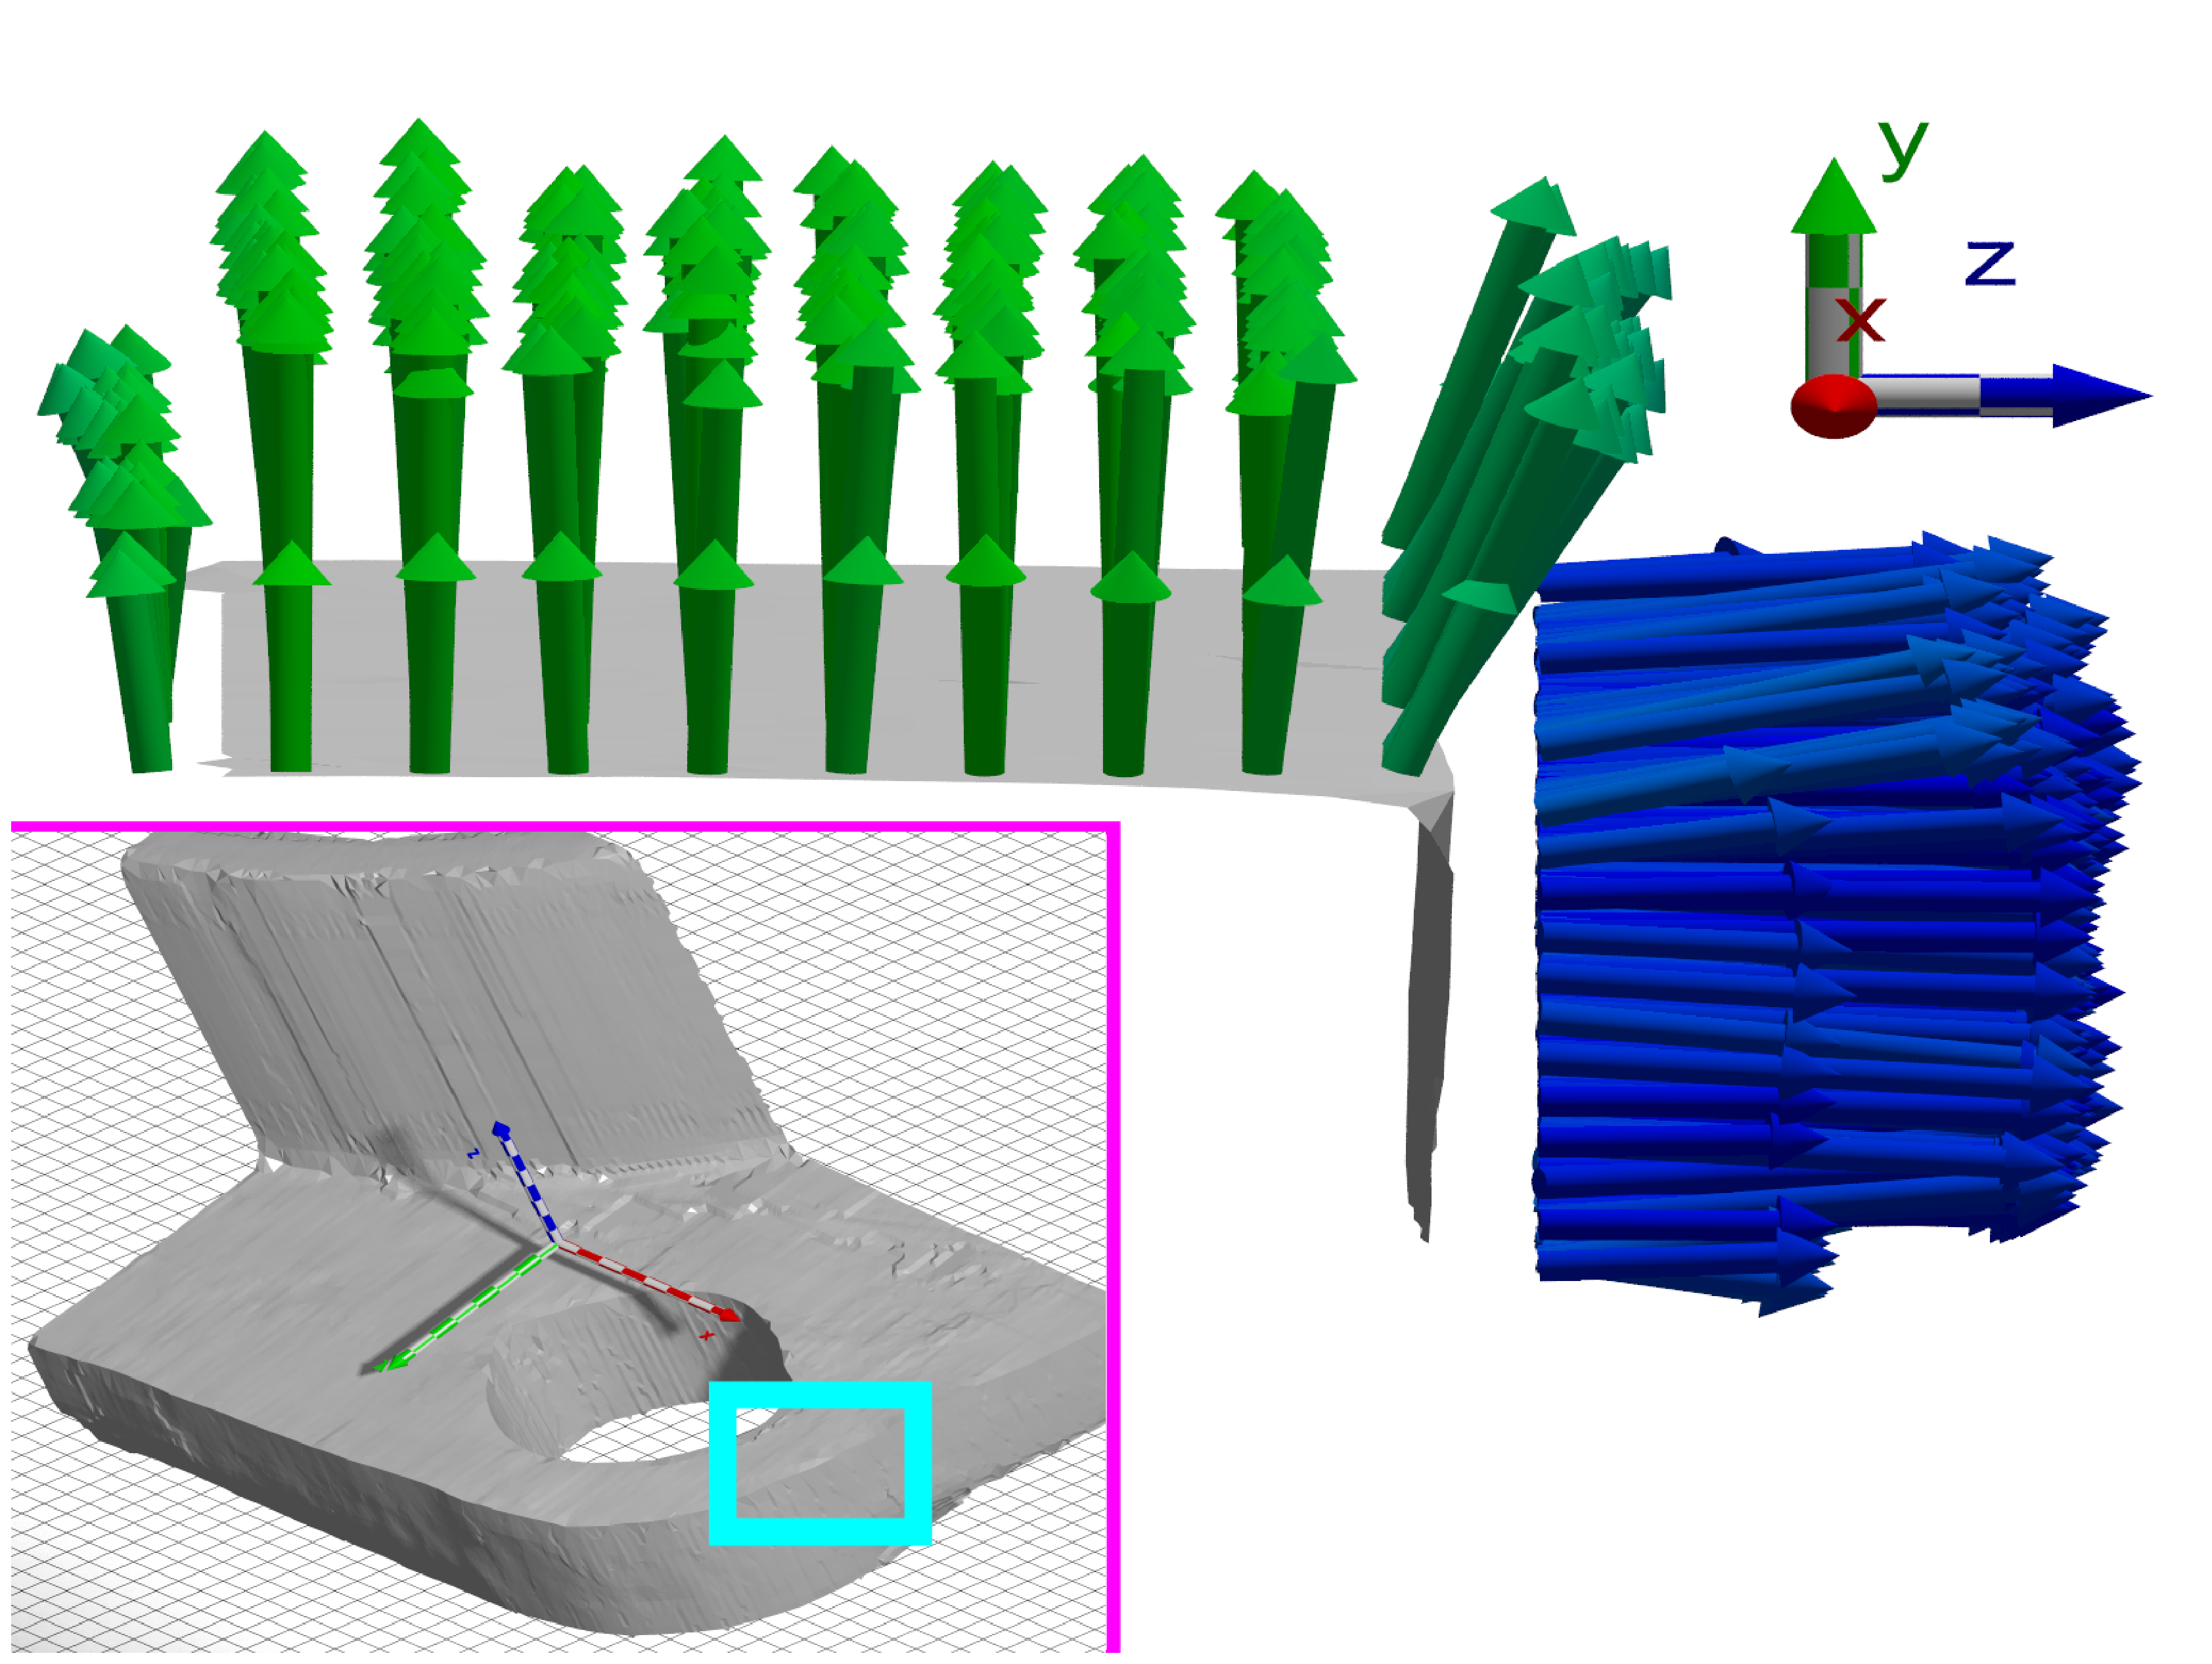
\includegraphics[width=0.5\linewidth]{images/setA.crop2.cdiff.new.eps}
	\caption{Gradient computation around a sharp surface edge in a CT data.
        Expanded view of the cyan rectangle, shows the central difference gradients at grid vertices which intersect the isosurface. Those parallel to Y axis are colored green, those parallel to Z are colored blue, the rest are linearly interpolated. The central difference formula produces incorrect gradients near the sharp edge. Gradients which are not near the sharp
        edge are correct.}
	\label{fig:grad-1}
    \end{center}
\end{figure}
\begin{figure}
	\centering
  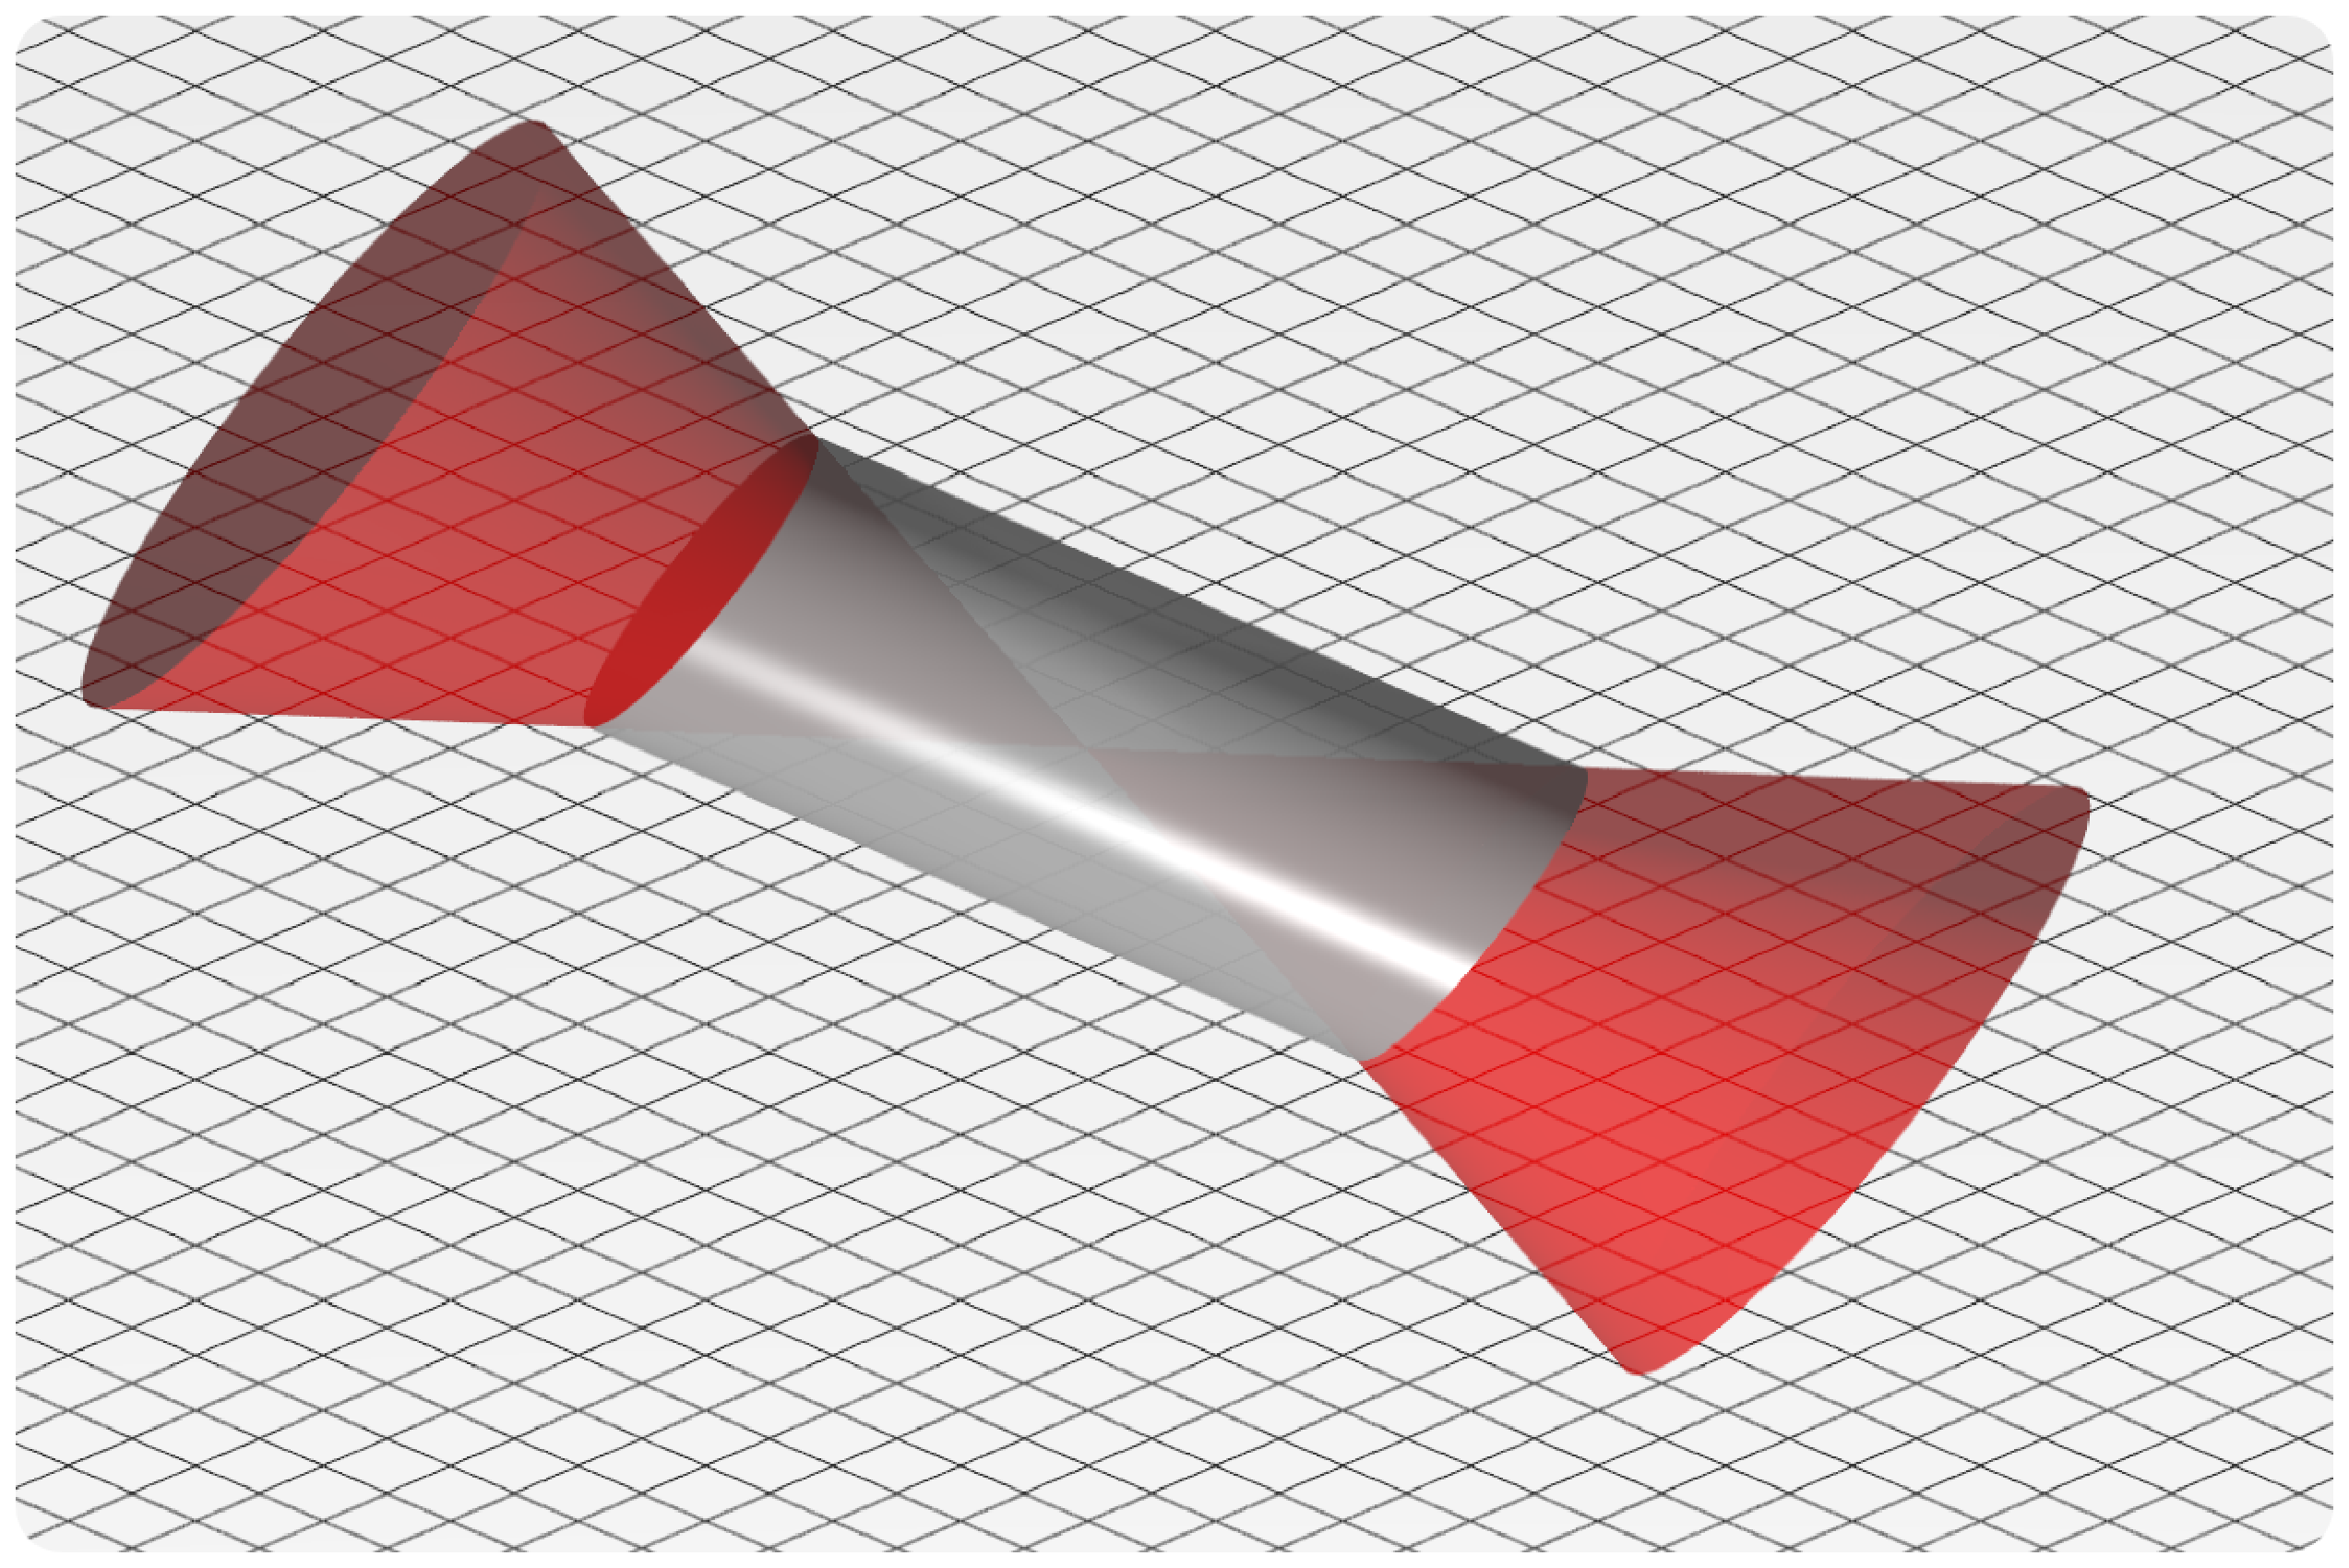
\includegraphics[width=0.5\linewidth]{images/2cone.eps}
  \caption{A double cone (red) representing the gradient discontinuities
 of a scalar field $f$.
 The field $f$ is the maximum of the distance to a line 
 and to a plane orthogonal to that line.
 The isosurfaces of $f$ are boundaries of cylinders.
 A sample isosurface is shown in grey.
 The double cone separates $\Rthree$ into three regions.
 The field $f$ is continuous within each region.}
	\label{fig:double_cone}
\end{figure}

%\begin{figure}[t]
%\begin{center}
%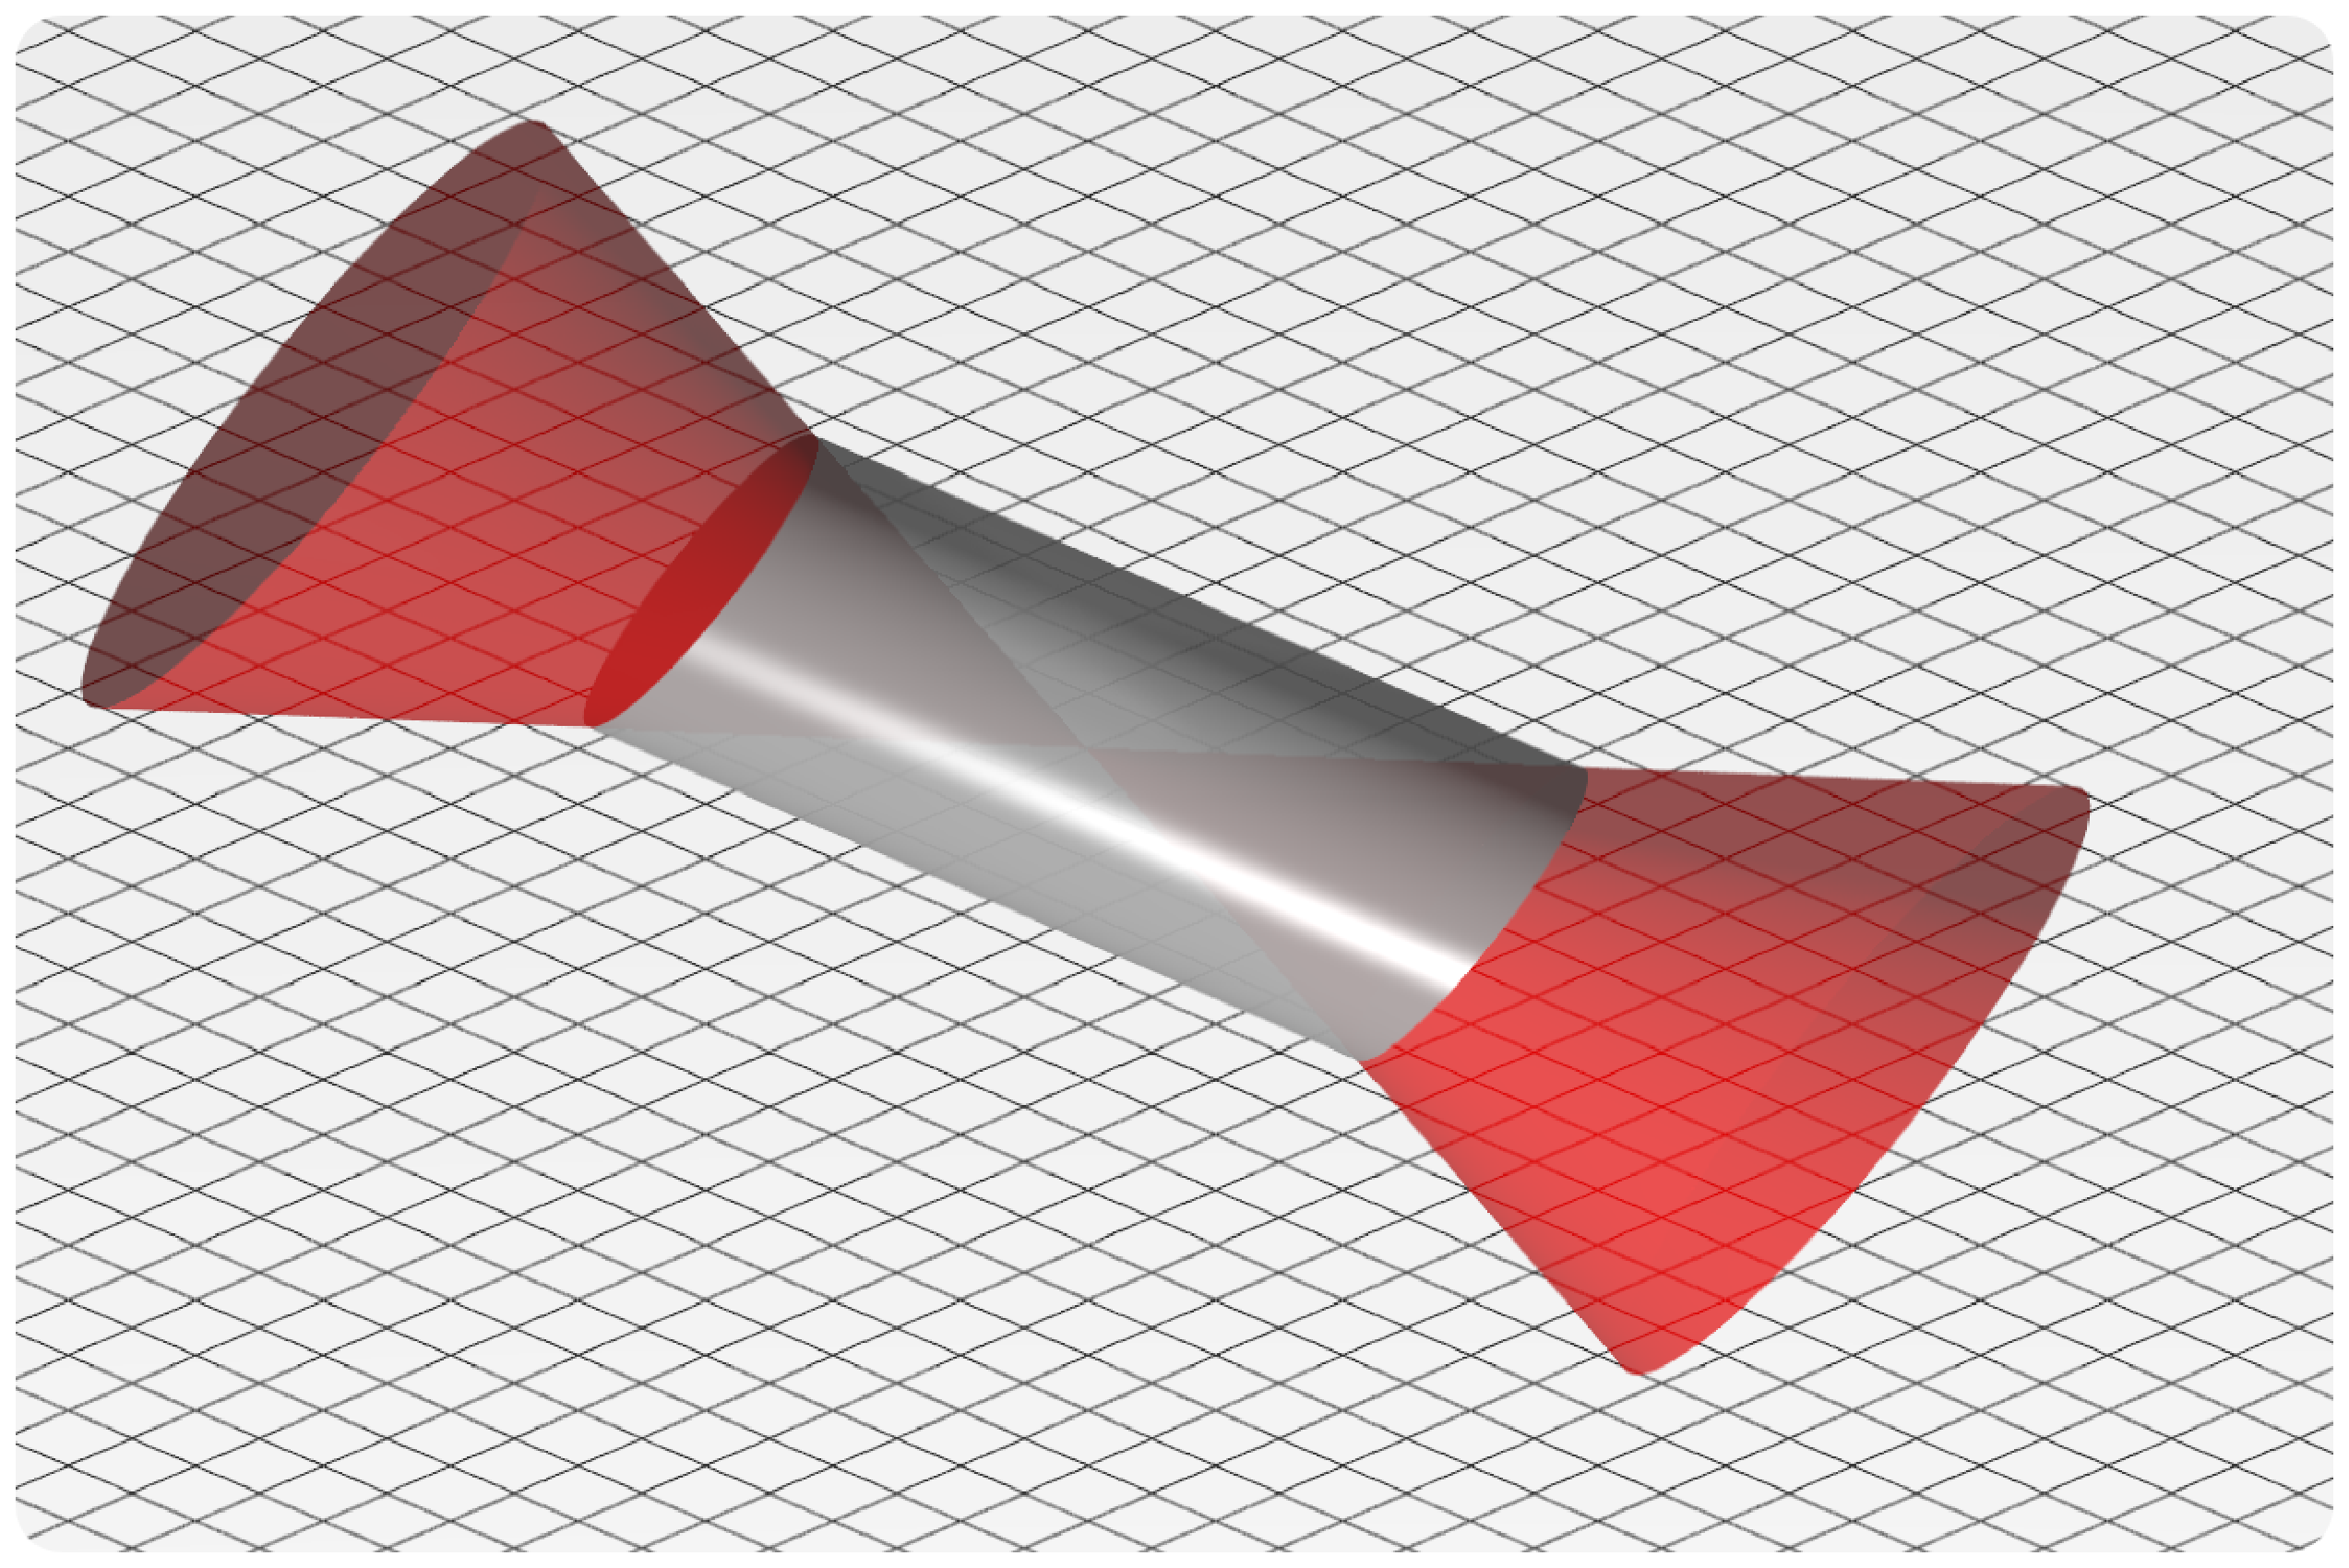
\includegraphics[width=\linewidth]{images/2cone.eps}
%\end{center}
%\caption{A double cone (red) representing the gradient discontinuities
%of a scalar field $f$.
%The field $f$ is the maximum of the distance to a line 
%and to a plane orthogonal to that line.
%The isosurfaces of $f$ are boundaries of cylinders.
%A sample isosurface is shown in green.
%The double cone separates $\Rthree$ into three regions.
%The field $f$ is continuous within each region.}
%\label{fig:double_cone}
%\end{figure}
\section{Determining Correct Gradients}
\label{sec:gradients}

We assume that the scalar values $s_v$ represent the values at the grid vertices $v$
of a continuous, piecewise smooth scalar field $f$. The difference between $s_v$ and $f(v)$ is the ``\textit{noise}'' in the data.

A scalar field $f :\Rthree \rightarrow \R$ is {\em piecewise smooth}
if $\Rthree$ can be partitioned into a finite set of piecewise smooth regions,
$A_1, A_2, \ldots, A_k$
such that $f$ has derivatives of all orders on each region $A_i$.
Because $f$ is only piecewise smooth,
the gradient field of $f$ may have discontinuities. Such discontinuities occur only on the boundaries, $\partial A_i$, 
of the $A_i$.

Figure~\ref{fig:double_cone} contains an example 
of a continuous piecewise smooth field,
consisting of three piecewise smooth regions
separated by two cones (a ``double cone'').
The isosurface for this field is the boundary of a cylinder.

The gradient at a point $p$ is the vector
$(\partial f/\partial x, \partial f/\partial y, \partial f/\partial z)$ at $p$.
Gradients are computed at some, but not all, of the grid vertices.
In particular, gradients are not computed at grid vertices \textit{on} 
or \textit{adjacent} to points where the scalar field is not smooth.

\subsection{Definitions}

We define the neighborhood of a grid vertex $v$.
Let set $N_1(v)$ be $v$ and the six grid vertices
which share a grid edge with $v$.
Recursively define set $N_k(v)$ as:
\begin{equation*}
N_k(v) = \{v': v' \in N_1(v'') \mbox{ for some } v'' \in N_{k-1}(v)\}.
\end{equation*}
We sometimes use $N(v)$ as an abbreviation for $N_1(v)$.

A {\em collinear sequence of adjacent grid vertices}
is a sequence $(v_1,v_2,\ldots,v_k)$ of distinct grid vertices
such that $v_i \in N(v_{i-1})$ for $i = 2,\ldots, k$
and all the $v_i$ are collinear.

An {\em interior grid vertex} of a region $A$
is a grid vertex $v$ such that $N(v)$ is a subset of $A$.
Set $\IV(A)$ is the set of all interior grid vertices of $A$.

%The {\em local feature size} of a point $p \in \XX$
%is the distance from $p$ to the medial axis of $\XX$.
%The local feature size is often used in analyzing 
%and proving the correctness of surface construction algorithms
%(e.g.~\cite{k-pgmls-08,dgqsww-fprss-12}.)


\subsection{Central Difference Formula}

To compute a gradient in a piecewise smooth scalar field,
we need all the scalar values used in the computation to be 
from a single smooth portion of the scalar field.
Thus, we want to use a small basis for our gradient computation
and not extend our gradient computation over many grid vertices.
We use the central difference formula
\begin{equation}
\partial f/\partial(x_d) \approx (f(x+u_d) - f(x-u_d))/(2|u_d|),
\label{eqn:cdiff}
\end{equation}
where $x$ is the location of a grid vertex and
$u_d$ is the vector to the adjacent vertex in direction $d$.
Figure~\ref{fig:grad-1} shows the result of computing
gradient using the central difference formula.

If spacing between grid vertices is the same in all directions,
then the grid can be rescaled so that $u_d$ is a unit vector 
in all directions.
However, CT scans often have non-uniform spacing,
with the $z$ or slice direction different from the $x$ and $y$ directions.
In that case, $u_x$ and $u_y$ will have different magnitudes from $u_z$.

Let $g_v$ be the gradient at a vertex $v$
and let $\tg_v$ be the gradient approximation produced 
by the central difference formula.
There are three types of errors in the approximation of $g_v$ by $\tg_v$.
First, there are errors caused by noise in the data,
i.e. the difference between the scalar value $s_v$ 
and it ``true'' value $f(v)$.
Second, there are errors caused by using the central difference formula
as an approximation to the gradient.
Such errors occur even if we used the exact values $f(v)$
and if the field was smooth everywhere.
Finally, if $v$ and one of its neighbors $v' \in N(v)$ 
lie in different smooth regions,
then there may be a discontinuity in the gradient along edge $(v,v')$.
This discontinuity will also contribute to errors in $\tg_v$. (Numerical error is a fourth contributor to errors in $\tg_v$,
but it is insignificant compared to the errors caused by noise in the data.)

Replacing the central difference formula by an equation 
which relies on more vertices will reduce the first two sources of error
but increase the effect of gradient discontinuities 
on the gradient approximation.
Anisotropic filtering can be used to decrease noise in the scalar data
without affecting the discontinuities,
but it will not reduce the error caused by gradient discontinuity.
Anisotropic filtering can also be used directly on the gradients.
Again, it will improve gradients in the smooth regions,
but it won't correct major errors caused by discontinuities.
(It might correct minor ones.)
\begin{figure}[t]
    \begin{center}
        \begin{tabular}{cc}
            \includegraphics[width=0.25\linewidth]{images/predicted.eps} \qquad &
            \qquad
            \includegraphics[width=0.25\linewidth]{images/predicted2.eps} \\
            (a) & (b)
        \end{tabular}
    \end{center}
    \caption{(a)~Vector $\phi(n,n')$ predicted by $n$ and $n'$.
        (b)~Vector $\phi_2(n,n')$ predicted by $n$ and $n'$.}
    \label{fig:predicted}
\end{figure}
%\begin{figure}[t]
%\begin{center}
%\begin{tabular}{cc}
%\includegraphics[width=1.4in]{images/predicted.eps} \qquad &
%\qquad
%\includegraphics[width=1.4in]{images/predicted2.eps} \\
%(a) & (b)
%\end{tabular}
%\end{center}
%\caption{(a)~Vector $\phi(n,n')$ predicted by $n$ and $n'$.
%(b)~Vector $\phi_2(n,n')$ predicted by $n$ and $n'$.}
%\label{fig:predicted}
%\end{figure}

\subsection{Reliable Gradients}
\label{sec:reliable}

For each vertex $v$, let $\tn_v = \tg_v/|\tg_v|$ be the unit vector
in the direction of the central difference gradient $\tg_v$.
We can try to determine if the gradient direction $\tn_v$ at vertex $v$ 
is reliable by comparing it with the gradient directions $\tn_{v'}$
at all the neighboring vertices $v' \in N(v)$.
If $\angle(\tn_v,\tn_{v'})$ is less than some constant $\alpha$ 
for all vertices $v' \in N(v)$,
then we can mark the gradient at $v$ as reliable.

Determining reliable gradients from $\angle(\tn_v,\tn_{v'})$
will work for flat regions but will fail if
the scalar field has any significant curvature.
If $\alpha$ is set to a small value,
then the algorithm will fail to detect correct gradients
in curved regions.
On the other hand, if $\alpha$ is set to a large value,
then the algorithm will mark incorrect gradients as correct.
Instead of comparing $\tn_v$ to neighboring vertices,
we use pairs of vertices to predict the gradient direction at $v$
and compare $\tn_v$ to this predicted direction.

Let $n_v = g_v/|g_v|$ be the unit vector pointing in the direction
of the true gradient $g_v$.
Assume $(v,v',v'')$ is a collinear sequence of adjacent vertices.
Vectors $n_v$ and $n_{v'}$ lie in a plane $h$.
If the gradient changes at a constant rate along line segment $(v,v'')$,
then $n_{v''}$ also lies in plane $h$ and 
$\angle(n_{v'},n_{v''})$ equals $\angle(n_v,n_{v'})$.

Let $n$ and $n'$ be unit vectors in $\Rthree$\
lying plane $h$.
Let $\phi(n,n')$ be the unit vector in $h$ other than $n$
whose angle with $n'$ is $\angle(n,n')$.
We say that the $\phi(n,n')$ is the vector 
{\em predicted by} $n$ and $n'$.
(See Figure~\ref{fig:predicted}(a).)
More precisely, define $\Orth(n,n')$ as $ n - (n \cdot n') n'$,
the component of $n$ orthogonal to $n$.
Define $\phi(n,n')$ as:
\begin{align*}
\phi(n,n') & = n - 2 \times \Orth(n,n') 
             = n - 2(n - (n \cdot n')n')
             = 2(n \cdot n') n' - n.
\end{align*}

As defined above, unit vector $\tn_v = \tg_v/|\tg_v|$
points in the direction of the central difference gradient.
We determine reliable gradients 
by testing $\angle(\phi(\tn_{v''},\tn_{v'}),\tn_v)$ against a constant $\alpha$.
\begin{algorithm}[h]
\Input{Vertex $v$, Angle bound $\alpha$.}
\BlankLine
\ForEach{grid vertex $v' \in N(v)$}{
Let $v'' \in N(v')$ be the vertex such that
$(v,v',v'')$ is a collinear sequence of adjacent vertices\;
\lIf{($\angle(\phi(\tn_{v''},\tn_{v'}),\tn_v) > \alpha$)}{\Return(\false)}
}
\Return(\true)
\caption{}
\label{alg:curved}
\end{algorithm}

Assume $N_3(v)$ is a subset of a smooth region $A_i$ 
so that $v, v', v'' \in \IV(A_i)$ for all the neighbors $v'$ of $v$.
If all the second order partial derivatives of function $f$ in $A_i$
are constant,
then the gradients change at a constant rate
along any direction and $\phi(n_{v''},n_{v'})$ equals $n_v$.
Moreover, if all the second order partial derivatives are constant
and there is no noise ($s_v = f(v)$ for all $v$),
then the central difference gradient $\tg_v$ 
equals the exact gradient $g_v$ (up to numerical error.)
(See Proposition~\ref{prop:cdiff} in the appendix for a proof.)

In the more general case, 
the second order partial derivatives are not constant 
and there is noise in the data.
To analyze this case, define:
\begin{align*}
& \mu = \max\{ \angle(n_v,\tn_v) : v \in \IV(A_i) \mbox{ for some } A_i \}.\\
& \Lambda(n_v,n_{v'},n_{v''}) = \angle(\phi(n_v,n_{v'}),n_{v''}).\\
& \lambda = \max\{ \Lambda(n_v, n_{v'},n_{v''}) :
                  v,v',v'' \in A_i \mbox{ for some } A_i \}.
\end{align*}
Value $\mu$ is a bound on the angle 
between the approximate and exact gradient directions
in the smooth regions of the field.
$\Lambda(n_v,n_{v'},n_{v''})$ is the difference 
between the prediction $\phi(n_v,n_{v'})$ and $n_{v''}$.
This difference is caused by changes in the curvature of $f$.
Value $\lambda$ is a bound on this difference 
over vertices in the interiors of the $A_i$.
Note that Algorithm~\ref{alg:curved} 
computes $\Lambda(\tn_{v''},\tn_{v'},\tn_v)$,
not $\Lambda(n_v,n_{v'},n_{v''})$.

The following proposition bounds $\Lambda(\tn_v,\tn_{v'},\tn_{v''})$
and $\angle(n_{v''},\tn_{v''})$.
\begin{proposition}
Let $(v, v', v'')$ be a collinear sequence of adjacent vertices
contained in $A_i$ for some smooth region $A_i$.
\begin{enumerate}
\item If $v, v', v'' \in \IV(A_i)$, then\\
{\centering
$\Lambda(\tn_v, \tn_{v'}, \tn_{v''}) \le 
\Lambda(n_v, n_{v'}, n_{v''}) + 4 \mu \le \lambda + 4 \mu$.}
\item If $v, v' \in \IV(A_i)$, then
$\angle(n_{v''},\tn_{v''}) \le 
   \Lambda(\tn_v,\tn_{v'},\tn_{v''}) + 3 \mu + \lambda$.
\end{enumerate}
\label{prop:angle}
\end{proposition}

\begin{proof}[Outline of proof of \ref{prop:angle}.1:]
Perturbing $n_v$ by at most $\mu$,
changes $\phi(n_v,n_{v'})$ by at most $\mu$.
Since angles $\angle(n_v,\tn_v)$ and $\angle(n_{v''},\tn_{v''})$
are at most $\mu$,
angle $\angle(\phi(\tn_v,\tn_{v'}), \tn_{v''})$ is at most
$\angle(\phi(n_v,\tn_{v'}), n_{v''})+2 \mu$.

Perturbing $n_{v'}$ by at most $\mu$
changes $\phi(n_v,n_{v'})$ by at most $2\mu$.
Thus,
\begin{align*}
\Lambda(\tn_v, \tn_{v'}, \tn_{v''}) & 
= \angle(\phi(\tn_v,\tn_{v'}), \tn_{v''}) \\
& \le \angle(\phi(n_v,\tn_{v'}), n_{v''}) + 2 \mu\\
& \le \angle(\phi(n_v,n_{v'}), n_{v''}) + 2 \mu + 2 \mu\\
& = \Lambda(n_v,n_{v'},n_{v''}) + 4 \mu.
\end{align*}
\end{proof}

\begin{proof}[Outline of proof of \ref{prop:angle}.2:]
By the triangle inequality,
\begin{align*}
\angle(n_{v''},\tn_{v''}) & \le 
\angle(\phi(n_v,n_{v'}),n_{v''}) + \angle(\phi(n_v,n_{v'}),\tn_{v''}) \\
& \le \lambda + \angle(\phi(n_v,n_{v'}),\tn_{v''}).
\end{align*}
As discussed above, perturbing $n_v$ by at most $\mu$
changes $\phi(n_v,n_{v'})$ by at most $\mu$.
Perturbing $n_{v'}$ by at most $\mu$
changes $\phi(n_v,n_{v'}$ by at most $2\mu$.
Thus,
\begin{align*}
\angle(n_{v''},\tn_{v''}) 
& \le \lambda + \angle(\phi(n_v,n_{v'}),\tn_{v''}) \\
& \le \lambda + \angle(\phi(\tn_v, \tn_{v'}), \tn_{v''}) + 3\mu \\
& = \Lambda(\tn_v,\tn_{v'},\tn_{v''}) + \lambda + 3\mu.
\end{align*}
\end{proof}
More complete versions of these proofs are in the appendix.

Assume that parameter $\alpha$ in Algorithm~\ref{alg:curved} 
is at least $\lambda + 4 \mu$.
By the first inequality, 
if $N_3(v) \subseteq A_i$ for some $A_i$,
then $\Lambda(\tn_{v''}, \tn_{v'}, \tn_v) \le \lambda+4\mu \le \alpha$
for all neighbors $v'$ of $v$.
Thus Algorithm~\ref{alg:curved} returns true.

On the other hand, assume that Algorithm~\ref{alg:curved} returns true
and that $N_3(v)$ intersects at most two regions.
Let $A_i$ be the region containing $v$.
Under the assumption that the boundary between these two regions is planar,
some $v' \in N(v)$ is in $\IV(A_i)$.
If $(v,v',v'')$ is a collinear sequence of adjacent vertices,
then $v''$ is also in $\IV(A_i)$.
By the second inequality,
$\angle(n_v,\tn_v) \le \Lambda(\tn_{v''},\tn_{v'},\tn_v) + 3 \mu + \lambda
\le \alpha + 3 \mu + \lambda$.
Thus, if Algorithm~\ref{alg:curved} returns true,
then the angle between the approximate gradient direction $\tn_v$
and the true gradient direction $n_v$
is bounded by $\alpha + 3\mu + \lambda$.
 \begin{figure}
	\centering
    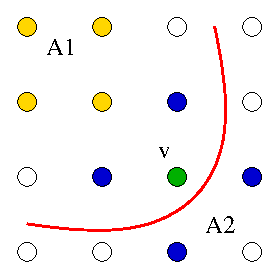
\includegraphics[width=0.5\linewidth]{images/curved_boundary.eps}
    \caption{Red curve is boundary separating regions $A_1$ and $A_2$.
        Green vertex $v$ is in $A_1$ but 
        no vertex of $N(v)$ lies in $\IV(A_1)$.
        Vertices in $N(v)$ are colored blue.
        Vertices in $\IV(A_1)$ are colored yellow.}
    \label{fig:curved_boundary}
    
 \end{figure}
    
%\begin{figure}
%	\centering
%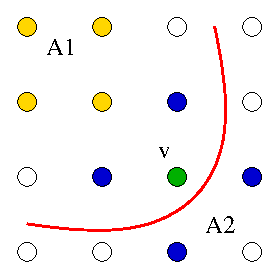
\includegraphics[width=0.25\linewidth]{images/curved_boundary.eps}
%	\caption{Red curve is boundary separating regions $A_1$ and $A_2$.
%           Green vertex $v$ is in $A_1$ but 
%           no vertex of $N(v)$ lies in $\IV(A_1)$.
%           Vertices in $N(v)$ are colored blue.
%           Vertices in $\IV(A_1)$ are colored yellow.}
%	\label{fig:curved_boundary}
%\end{figure}

So far we've made the assumption that the surface
between two smooth regions is planar.
If we drop that assumption, then it is no longer true
that for every vertex $v \in A_i$ some vertex in $N(v)$ is in $\IV(A_i)$.
For instance, in the 2D example in Figure~\ref{fig:curved_boundary},
no vertex in $N(v)$ lies in $\IV(A_1)$.
Without this property, we can no longer guarantee a bound
on $\angle(n_v, \tn_v)$ when Algorithm~\ref{alg:curved} returns true.

To handle curved boundaries of the $A_i$,
we must modify our algorithm to use vertices 
at edge distance 3 from $v$.
We define $\phi_k(n_v,n_{v'})$ as the normal direction 
predicted by $n_v$ and $n_{v'}$ at the vertex 
which is edge distance $k$ from $n_{v'}$.
\begin{align*}
\phi_0(n,n') & = n', \\
\phi_1(n,n') & = \phi(n,n') = 2 (n \cdot n') n' - n, \\
\phi_k(n,n') & = \phi(\phi_{k-2}(n,n'),\phi_{k-1}(n,n')), \\
\Lambda_k(n,n',n'') & = \angle(\phi_k(n,n'),n'').
\end{align*}

We replace $\phi$ in Algorithm~\ref{alg:curved} with $\phi_2$.
\begin{algorithm}[h]
\Input{Vertex $v$, Angle bound $\alpha$.}
\BlankLine
\ForEach{grid vertex $v' \in N(v)$}{
Let $v'',v''' \in N_3(v)$ be the vertices such that
$(v,v',v'',v''')$ is a collinear sequence of adjacent vertices\;
\lIf{($\angle(\phi(\tn_{v''},\tn_{v'}), \tn_v) > \alpha$)}{\Return(\false)}
\lIf{($\angle(\phi_2(\tn_{v'''},\tn_{v''}), \tn_v) > \alpha$)}
{\Return(\false)}
}
\Return(\true)
\caption{}
\label{alg:phi2}
\end{algorithm}

Let $A_i$ be the smooth region containing vertex $v$.
Let $\XX = \cup_{A_j} \partial A_j$ be the union of all the boundaries
of smooth regions $A_j$.
If there is a sufficiently large ball containing $v$
and not intersecting $\XX$, then $v'',v''' \in \IV(A_i)$
for some collinear sequence $(v,v',v'',v''')$.
\begin{proposition}
Let $\Gamma$ be a regular grid whose edges all have the same length $L$.
If some ball $\BB$ of radius $(5/2)\sqrt{3}L$ contains grid vertex $v \in A_i$
and does not intersect $\XX$,
then there is a collinear sequence $(v,v',v'',v''')$ 
of adjacent grid vertices 
such that $v'' \in \IV(A_i)$ and $v''' \in \IV(A_i)$.
\label{prop:IV}
\end{proposition}

To prove Proposition~\ref{prop:IV}, 
we show that there $\BB$ contains $N_v(v'')$ and $N_v(v''')$
for some collinear sequence $(v,v',v'',v''')$.
The proof is in the appendix.

The following proposition bounds $\Lambda_2(\tn_v,\tn_{v'},\tn_{v'''})$
and $\angle(n_{v'''},\tn_{v'''})$.
\begin{proposition}
Let $(v, v', v'',v''')$ be a collinear sequence of adjacent vertices
contained in $A_i$ for some smooth region $A_i$.
\begin{enumerate}
\item If $v, v', v'', v''' \in \IV(A_i)$, then\\
{\centering
$\Lambda_2(\tn_v, \tn_{v'}, \tn_{v'''}) \le 
\Lambda_2(n_v, n_{v'}, n_{v'''}) + 6 \mu \le 3\lambda + 6 \mu$.}
\item If $v, v' \in \IV(A_i)$, then\\
{\centering
$\angle(n_{v'''},\tn_{v'''}) 
   \le \Lambda(\tn_v,\tn_{v'},\tn_{v'''}) + 3\lambda+ 5 \mu$.}
\end{enumerate}
\label{prop:angle:b}
\end{proposition}
Proofs of these relationships are in the appendix.

As in the discussion, of Algorithm~\ref{alg:curved},
Property~\ref{prop:angle:b} can be used to show that 
if $N_4(v) \subset A_i$ for some $A_i$,
then Algorithm~\ref{alg:phi2} returns true.
On the other hand, assume Algorithm~\ref{alg:phi2} returns true.
By Proposition~\ref{prop:IV},
there is a collinear sequence of grid vertices $(v,v',v'',v''')$
such that $v'',v''' \in \IV(A_i)$.
By Proposition~\ref{prop:angle:b},
the angle between the approximate gradient direction $\tn_v$
and the true gradient direction $n_v$ is bounded by $\alpha + 3\lambda + 5 \mu$.

%The condition that a ball $\BB$ of radius $(5/2)\sqrt{3}$ 
%contains $v$ and does not intersect $\XX$
%can be formulated as a lower bound on the local feature size of $\XX$
%in the neighborhood of $v$.
%A lower bound on the local feature size of $\XX$ near $v$
%implies an upper bound on the curvature of $\XX$ near $v$.
%
%If the edge lengths of grid $\Gamma$ are not equal,
%then ball $\BB$ can be replaced by a suitable ellipsoid
%to give similar conditions for $v''$ and $v'''$ to be in $\IV(A_i)$.

\begin{algorithm}[h]
\NoLineNum{\DoesOrthMatchA{$v$, $\alpha_1$, $\alpha_2$}}
\lIf{($N^O(v) = \emptyset$)}{ \Return(\true)}
\ForEach{grid vertex $v' \in N^O(v)$}{
Let $v'',v''' \in N_3(v)$ be the vertices such that
$(v,v',v'',v''')$ is a collinear sequence of adjacent vertices
$\flagMatch \leftarrow \false$\;
\lIf{($\angle(\tn_v, \phi(\tn_{v''},\tn_{v'})) \le \alpha_2$) \KwAnd \\
     \hspace{1em} 
     ($\angle(\tn_v, \phi_2(\tn_{v'''},\tn_{v''})) \le \alpha_2$)}{
$\flagMatch \leftarrow \true$
}
\lIf{($\angle(\tn_v, \tn_{v'}) \le \alpha_1$) \KwAnd \\
    \hspace{1em} ($\angle(\tn_v, \tn_{v''}) \le \alpha_1$)}{
$\flagMatch \leftarrow \true$
}
\lIf{($\flagMatch = \false$)}{ \Return(\false) }
}
\Return(\true)
\caption{Algorithm \protect\DoesOrthMatchA.}
\label{alg:orthA}
\end{algorithm}
\begin{algorithm}[h]
\NoLineNum{\DoesOrthMatchB{$v$, $\alpha_1$}}
\ForEach{grid vertex $v' \in N^O(v)$}{
\If{($v \in N^O(v')$)}{
\lIf{($\angle(\tn_v,\tn_{v'}) \le \alpha_1$)}
{\Return(\true)}
}
}
\Return(\false)
\caption{Algorithm \protect\DoesOrthMatchB.}
\label{alg:orthB}
\end{algorithm}

\begin{algorithm}[h]
\NoLineNum{\FindReliable{$v$, $\alpha_1$, $\alpha_2$}}
\tcc{$\alpha_1$ and $\alpha_2$ are angle bounds}
\ForEach{grid vertex $v' \in N^T_v$}{
Let $v'',v''' \in N_3(v)$ be the vertices such that
$(v,v',v'',v''')$ is a collinear sequence of adjacent vertices\;
\lIf{($\angle(\tn_v, \phi(\tn_{v''},\tn_{v'})) > \alpha_2$)}{\Return(\false)}
\lIf{($\angle(\tn_v, \phi_2(\tn_{v'''},\tn_{v''})) > \alpha_2$)}
{\Return(\false)}
}
\lIf{\DoesOrthMatchA($v$, $\alpha_1$, $\alpha_2$)}
{ \Return(\true) }
\lElseIf{\DoesOrthMatchB($v$, $\alpha_1$)}
{ \Return(\true)}
\lElse{ \Return(\false)}
\caption{Algorithm \protect\FindReliable}
\label{alg:phi3}
\end{algorithm}



\subsection{CT Data}

Algorithm~\ref{alg:phi2} has two problems when applied to CT data.
First, 
in CT data scalar values near gradient discontinuities
are very unreliable.
At such vertices, the angle between the true gradient $n_v$
and the estimated gradient direction $\tn_v$ is also very unreliable.
Thus, we cannot assume that angle is bounded by a constant $\mu$
on vertices near gradient discontinuities.
Second, gradient magnitudes drop off quickly away from the surface boundaries
and gradient directions are quickly meaningless.
This is particularly true if the gradient direction is the z-direction
and the CT data is reconstructed in planar x-y slices.
We address each of these problems.

The first problem with CT data is that scalar values near gradient
discontinuities are very unreliable.
At such vertices,
the angle between $n_v$ and $\tn_v$ can be much greater 
than in the rest of the data set.
Unfortunately, gradients at vertices near gradient discontinuities 
are exactly the gradients which we need to generate sharp features.

Gradients generated from scalar data rely upon the accuracy
of the scalar data.
CT scanners do not measure scalar values directly at each grid vertex.
Instead, they measure the intensity of rays passing 
through the scanned object.
The resulting measurements are called projection data.
The projection data is transformed into scalar data
by using a Radon or similar transformation
of by solving a large set of linear equations.
The resolution of the scalar data is usually set to equal
the resolution of the projection data.

The process of determining scalar values at grid vertices
is provably reliable in regions where field gradients 
vary slowly and continuously.
However, it is highly unreliable near discontinuities 
in the field gradients.
The result is that scalar values at grid vertices
adjacent to gradient discontinuities are highly unreliable
and the angle between the true gradient and the estimated gradient
can be much larger than in the rest of the data.

Fortunately, the scalar errors drop off quickly away 
from the gradient discontinuities.
We found that scalar values at a grid vertex $v$ was reliable
within an acceptable tolerance as long as no edge incident on $v$
intersected a gradient discontinuity.
Equivalently, the scalar value at $v \in A_i$ was reliable
as long as $N(v)$ was a subset of $A_i$.
Under this assumption,
if $N_2(v)$ is contained in some smooth region $A_i$,
then the scalar values at vertices in $N(v)$ are close to their true values.
This implies that the angle between $n_v$ and $\tn_v$ is small.

Let $A_i$ be the smooth region containing grid vertex $v$.
Assume that the boundary of $A_i$ is flat around $v$.
We can no longer assume that the angle between $n_{v'}$ and $\tn_{v'}$
is small for some $v' \in N(v)$.
However, there is a collinear sequence $(v,v',v'',v''')$ 
of adjacent vertices such that $N_2(v'')$ and $N_2(v''')$ 
are in $A_i$.
Thus, $\tn_{v''}$ and $\tn_{v'''}$ are good estimates
of $n_{v''}$ and $n_{v'''}$, respectively.
By comparing $\tn_v$ with the direction $\phi_2(\tn_{v'''},\tn_{v''})$
predicted by $\tn_{v'''}$ and $\tn_{v''}$,
we can determine if $\tn_v$ is a reliable gradient.
Note that this exactly what Algorithm~\ref{alg:phi2} does.

The argument above assumes the boundary of $A_i$ is flat around $v$.
Without this assumption, we can no longer conclude that $N_2(v'')$
and $N_2(v''')$ are in $A_i$ for some collinear sequence $(v,v',v'',v''')$.

Assume that all grid edges have the same length $L$.
Replace the assumption that a scalar value at $v \in A_i$ is reliable
if $N(v) \subseteq A_i$
by the assumption that a scalar value at $v$ is reliable
if a ball $\BB_{0.5L}(v)$ of radius $0.5L$ around $v$ 
is contained in $A_i$.
Under this assumption,
if $\BB_{1.5L}(v)$ is contained in some smooth region $A_i$,
then the scalar values at the vertices $N(v)$ 
are all close to their true values.
This implies that the angle between $n_v$ and $\tn_v$ is small.

If $\BB'$ is a sufficiently large ball containing $v$ and $A_i$
contains $\BB'$,
then there is a collinear sequence $(v,v',v'',v''')$ 
of adjacent grid vertices 
such that $A_i$ contains $\BB_{1.5}(v'')$ and $\BB_{1.5}(v''')$.
Thus, $\tn_{v''}$ and $\tn_{v'''}$ are reliable gradients.
Algorithm~\ref{alg:phi2} determines if $\tn_v$ is reliable
from $\tn_{v''}$ and $\tn_{v'''}$.

The second problem with CT data is that gradient magnitudes 
drop off quickly away from the surface boundaries.
To address this problem,
we divide the vertex neighbors of $v$ into two sets.
Define the the tangent neighbor set and
the orthogonal neighbor set of $v$ as:
\begin{align*}
N^T(v) & = \{ v' \in N(v) : 
  20^\circ \le \angle(\tn_v,(v'-v)) \le 160^\circ. \} \\
N^O(v) & = N(v) - N^T_v \\
       & = \{ v' \in N(v) : \angle(\tn_v,(v'-v)) < 20^\circ \mbox{ or } \\
       & \qquad \qquad \angle(\tn_v,(v-v')) < 20^\circ. \}
\end{align*}
$(v'-v)$ is the vector from $v$ to $v'$.
The orthogonal neighbor set may be empty.

Assuming that $\tn_v$ is relatively close to $n_v$,
vertices in $N^T(v)$ are near the tangent plane at $v$
and close to the isosurface through $v$.
We handle gradient directions at those vertices as in Algorithm~\ref{alg:phi2}.
Vertices in $N^O(v)$ are (relatively) far from the tangent plane
and from the isosurface through $v$.
Fortunately, the gradient directions at the vertices in $N^O(v)$
are much more reliable than the gradient directions at vertices in $N^T(v)$.
Thus, we can use gradients at vertices in $N^O(v)$ 
to determine whether gradient $\tn_v$ is reliable.
We reduce the number of nearby vertices whose gradient directions
must match $\tn_v$ in three ways.

First, we note that there is little curvature along the gradient direction
in the scalar field represented by a CT scan.
Thus, in addition to the comparison 
of $\tn_v$ and $\phi_2(\tn_{v'''},\tn_{v''})$,
we can simply compare $\tn_v$ and $\tn_{v''}$.
If angle $\angle(\tn_v,\tn_{v''})$ is below some threshold $\alpha_1$,
then $\tn_{v''}$ can be a guarantor of the reliability of $\tn_v$.
(See Algorithm~\ref{alg:orthA}.)

Second, instead of comparing $\tn_v$ and $\tn_{v''}$,
we compare $\tn_v$ to its immediate neighbor $\tn_{v'} \in N(v)$
(Algorithm~\ref{alg:orthB}.)
We still compare $\tn_v$ with vertices at edge distance 3
in the tangent directions.
If some sufficiently large ball contains $v \in A_i$
and does not intersect $\XX = \cup_{A_j} \partial A_j$,
then either there is a $v' \in N^T(v)$ and collinear sequence $(v,v',v'',v''')$
where $v'',v''' \in \IV(A_i)$
or there is a $v' \in N^O(v)$ such that $v' \in \IV(A_i)$.

Third, in Algorithm~\ref{alg:orthB}
we replace the requirement that gradient directions 
of both vertices in $N^O(v)$ ``match'' $\tn_v$
by a requirement that the gradient direction of one vertex
in $N^O(v)$ matches $\tn_v$.
Let $N^O(v) = \{v'_1, v'_2\}$.
We require that either the $\angle(\tn_v, \tn_{v'_1})$ 
or that $\angle(\tn_v, \tn_{v'_2})$  is small.
To make sure that we are only applying the single check
to gradients which truly point along an axis,
we require also that $\tn_{v'_1}$ or $\tn_{v'_2}$
be close to the axis direction.

Algorithm~\ref{alg:orthA} contains the check
in both orthogonal directions.
Algorithm~\ref{alg:orthB} contains the additional check 
in one orthogonal direction.
Because of the check $v \in N^O(v')$ in line 2 of Algorithm~\ref{alg:orthB},
there are cases where Algorithm~\ref{alg:orthA} may return true
while Algorithm~\ref{alg:orthB} returns false.
Algorithm~\ref{alg:phi3} is the full algorithm.

Algorithm~\ref{alg:phi3} loosens the conditions 
under which a gradient is identified as reliable.
By Proposition~\ref{prop:angle:b},
if $N_4(v) \subset A_i$ for some $A_i$,
then Algorithm~\ref{alg:phi3} returns true.
What about the converse, i.e. if Algorithm~\ref{alg:phi3} returns true?

We can show that for each $v \in A_i$,
there is either a collinear sequence of grid vertices $(v,v',v'',v''')$
such that $v' \in N^T(v)$ and $v'',v''' \in \IV(A_i)$
or there is a vertex $v' \in N^O(v)$ such that $v' \in \IV(A_i)$.
(See Proposition~\ref{prop:IV:b} in the appendix.)
In the first case,
the angle between the approximate gradient direction $\tn_v$
and the true gradient direction $n_v$ is bounded 
by $\alpha_2 + 3\lambda + 5 \mu$.
In the second case,
the angle between $\tn_v$ and $n_v$ is bounded by
$\angle(\tn_v,\tn_{v'}) + \kappa + \mu$
where $\kappa$ is a bound on curvature.
(See Prop~\ref{prop:kappa} in the appendix.)
If $\angle(\tn_v,\tn_{v'}) \le \alpha_1$,
then $\angle(\tn_v,n_v) \le \alpha + \kappa + \mu$.
However, Algorithm \DoesOrthMatchB (Algorithm~\ref{alg:orthB}),
only guarantees that $\angle(\tn_v, \tn_w) \le \alpha_1$
for one vertex $w \in N^O(v)$.
What if $w$ is not the vertex of $N^O(v)$ which is in $\IV(A_i)$?

We think that if $\angle(\tn_v,\tn_w) \le \alpha_1$ for one $w \in N^O(v)$
and $\angle(\tn_v,\phi_2(\tn_{w'''},\tn_{w''})) \le \alpha_2$
for all collinear sequences $(v,w',w'',w''')$ where $w' \in N^T(v)$,
then $\angle(\tn_v, n_v)$ is small.
However, we don't yet have a proof.


\begin{algorithm}[h]
\NoLineNum{\ExtendReliable{$\alpha_2$, $\numIter$}}
\For{$k \leftarrow 1$ \KwTo $\numIter$}{
$S \leftarrow \emptyset$\;
\ForEach{vertex $v$}{
\ForEach{vertex $v' \in N^T(v)$}{
Let $v'',v''' \in N_3(v)$ be the vertices such that
$(v,v',v'',v''')$ is a collinear sequence of adjacent vertices\;
\If{($v'$, $v''$ and $v'''$ are marked reliable)}{
\If {($\angle(\tn_v,\phi(\tn_{v''},\tn_{v'})) < \alpha_2$) \KwAnd
     ($\angle(\tn_v,\phi_2(\tn_{v'''},\tn_{v''})) < \alpha_2$)}
{ $S \leftarrow S \cup \{v\}$\; }
}
}
}
Mark each vertex $v \in S$ as reliable\;
}
\caption{Algorithm \protect\ExtendReliable}
\label{alg:extend}
\end{algorithm}

\subsection{Extending Reliable Gradients}
\label{sec:extendGrad}
Once we've identified reliable gradients by Algorithm~\ref{alg:phi3},
we can use those reliable gradients to identify vertex neighbors
with reliable gradients.
By Proposition~\ref{prop:angle:b},
if $v''$ and $v'''$ are reliable and 
$\angle(\phi_2(\tn_{v'''},\tn_{v''}), \tn_v)$ is small,
then $\angle(\tn_v, n_v)$ is small.
This is particularly helpful near gradient discontinuities,
where Algorithm~\ref{alg:phi3} will fail to identify correct gradients
as reliable because some of their neighbors are incorrect.

Pseudo code for Algorithm~\ExtendReliable is given 
in Algorithm~\ref{alg:extend}.
Because the initial set of reliable gradients is computed
If the initial set of reliable gradients is computed using $(v,v',v'',v''')$,
the value of $\numIter$ is set to 2.

\begin{algorithm}[h]
\NoLineNum{\ReliGrad{$\alpha_1$, $\alpha_2$, $\numIter$}}
\lForEach{grid vertex $v$}{
\FindReliable{$v$,$\alpha_1$,$\alpha_2$}
}
\ExtendReliable{$\alpha_2$, $\numIter$}
\BlankLine
\caption{Algorithm \protect\ReliGrad}
\label{alg:religrad}
\end{algorithm}

\subsection{Algorithm \protect\ReliGrad}
\label{sec:ReliGrad}

Our final algorithm, named \ReliGrad, applies Algorithm~\FindReliable
to each vertex and then calls \ExtendReliable.
Pseudo code is in Algorithm~\ref{alg:religrad}.

